\chapter{Entorno de experimentación} \label{chapter:chapter3}

\section{Análisis y procesamiento del corpus}

Siendo el objetivo de este trabajo la evaluación de un método semi-supervisado aplicado al reconocimiento de entidades nombradas se hizo necesario contar con un corpus para realizar dicha tarea. Por ello, se decidió utilizar a WiNER , un corpus anotado a partir de artículos de la Wikipedia en inglés construido en el trabajo de \cite{WiNER-Ghaddar-Langlais}.

Dicho corpus consta de 3.2M de artículos de Wikipedia, que comprende más de 54M de oraciones, de las cuales 41M contienen al menos una anotación de entidad nombrada, generando un total de 106M de anotaciones (un promedio de 2 entidades por oración).

Los tipos de entidades anotadas en este conjunto de datos son PER, LOC y ORG que denotan nombres de personas, lugares y organizaciones respectivamente. También se cuenta con la etiqueta MISC, categoría que incluye aquellas entidades no pertenecientes a las categorías anteriormente mencionadas. \textit{Agatha Christie} (PER), \textit{Belgian} (LOC), \textit{Warner Bros} (ORG) y \textit{Black Coffee} (MISC) son algunos ejemplos de entidades nombradas de este corpus. En caso de que no se trate de una instancia que no corresponde a una entidad nombrada se utiliza, por convención, la etiqueta O.

Una de las primeras decisiones tomadas durante el procesamiento del corpus fue considerar entidades cuya cardinalidad a nivel de palabra fuese uno. Esto se logró separando aquellas entidades formadas por más de una palabra en nuevas entidades donde a cada palabra le corresponde el mismo tipo de entidad de la cual fue separada. En el ejemplo anterior de \textit{Agatha Christie}, ahora se considera \textit{Agatha} y \textit{Christie} como dos entidades independientes, ambas del tipo PER.

El corpus contiene un total de 3223 documentos. El Cuadro \ref{tab:division} muestra la división de datos para conformar los conjuntos de entrenamiento, evaluación y validación.

\begin{table}[ht]
    \centering
    \begin{tabular}{|c|c|}
        \hline
        \textbf{Corpus} & \textbf{Documentos} \\
        \hline \hline
        Entrenamiento & 0 - 1999 \\
        Validación & 2000 - 2599 \\
        Evaluación & 2600 - 3223 \\
        \hline
    \end{tabular}
    \caption{División de los datos para entrenamiento, validación y evaluación.}
    \label{tab:division}
\end{table}

A partir de esa división se tomaron a su vez muestras aleatorias de cada conjunto de documentos detallados en el Capítulo \ref{chapter:chapter4}. Esto fue necesario por cuestiones de limitación de recursos computacionales y tiempo para la ejecución de los distintos experimentos. Se realizó un preprocesamiento sobre los 3223 documentos, cada uno de estos documentos tiene asociado aproximadamente 1000 artículos identificados con un número único. Para cada artículo existe entonces un archivo asociado cuya primera línea tiene su wikiID seguidos de sus oraciones una por línea. En los artículos, los tokens (palabras, símbolos, signos, etc.) están representados por un ID unívoco.

\paragraph{Ejemplo}\hfill

\vspace{0.5em}

\begin{tabular}{|l|}
    \hline
    63903 24730 9 7 3035 4104 7584 1 355 17 22825 9984 2 \\
    \hline
\end{tabular}

\vspace{0.5em}

Es equivalente a:

\begin{tabular}{|l|}
    \hline
    Hercule Poirot is a fictional Belgian detective , created \\
    by Agatha Christie . \\
    \hline
\end{tabular}

\vspace{1em}

Gracias a esta metodología de almacenamiento del corpus no fue necesario aplicar ningún tokenizador sobre el texto. A su vez, se decidió no remover signos de puntuación al igual que las palabras más comunes del idioma \textit{stopwords} con la premisa de que en el caso de removerlas se perdería información útil sobre el contexto de cada palabra para nuestra tarea particular de reconocimiento de entidades nombradas. Una vez realizada la transformación y obtenidas las oraciones, se construyeron las distintas instancias de entrenamiento que se mencionan en la sección \ref{sec:instanciasEntrenamiento}. Finalmente, se encuentran codificadas las entidades de cada artículo. El formato es el siguiente:

\vspace{0.5em}

\begin{tabular}{|l|}
    \hline
    ID $<$wikiID$>$ \\
    sentIdx begin end entityType \\
    \hline
\end{tabular}

\vspace{1em}

Donde \textit{sentIdx} representa el número de oración del artículo, \textit{begin} la posición donde comienza una entidad en la oración, \textit{end} la posición donde termina y \textit{entityType} el tipo de entidad que se trata:

\vspace{0.5em}

\begin{tabular}{|ll|}
    \hline
    entityType[0] = PER & entityType[1] = LOC \\
    entityType[2] = ORG & entityType[3] = MISC \\
    \hline
\end{tabular}

\vspace{1em}

Continuando el ejemplo anterior:

\vspace{0.5em}

\begin{tabular}{|llll|}
    \hline
    ID & 1000 & & \\
    0 & 0 & 2 & 0 \\
    0 &	5 &	6 & 1 \\
    0 &	10 & 12 & 0 \\
    \hline
\end{tabular}

\vspace{1.0mm}

Resulta en:

\vspace{0.5em}

\begin{tabular}{|l|}
    \hline
    [Hercule Poirot]$_{PER}$ is a fictional [Belgian]$_{LOC}$ detective , \\
    created by [Agatha Christie]$_{PER}$ . \\
    \hline
\end{tabular}

\section{Instancias de entrenamiento}
\label{sec:instanciasEntrenamiento}

En este trabajo se exploraron tres maneras de representar a los datos en los
modelos de aprendizaje.

\subsection{Palabra - etiqueta}\label{sec:palabraEtiqueta}

En este caso se hizo necesario investigar metodologías que nos permitieran representar a una palabra teniendo el cuenta el contexto en el cual ocurre. Como primera medida, se decidió utilizar los \textit{embeddings} pre-entrenados de Google\footnote{\url{https://code.google.com/archive/p/word2vec/}} para transformar a cada palabra en un vector que la representa en un espacio de dimensionalidad igual a 300.

Siguiendo el trabajo de \cite{iacobacci-etal-2016-embeddings} se exploraron cuatro estrategias distintas para obtener una representación más informativa de cada palabra.

\subsubsection{Concatenación}
Este método consiste en concatenar los vectores de palabras que rodean una palabra objetivo en un vector más grande, que tiene un tamaño igual a las dimensiones sumadas de todas las proyecciones (\textit{embeddings}) individuales.

\begin{itemize}
    \item $w_{ij}$ = peso asociado con la i-ésima dimensión del vector de la j-ésima palabra en la oración. Con los vectores de palabras de una oración se forma una matriz $w^{\space D\space x\space L}$ donde $L$ es la cantidad de palabras de esa oración.
    \item $D$ = dimensionalidad de los word vectors originales. Por ejemplo, al usar el modelo Word2Vec de Google se tiene $D$ = 300.
    \item $W$ = tamaño de ventana que se define como el número de palabras en un solo lado.
\end{itemize}

Nos interesa representar el contexto de la I-ésima palabra de la oración. La i-ésima dimensión del vector de concatenación, que tiene un tamaño de $2 W D$, se calcula de la siguiente manera:

$$e_{i} =\begin{cases} 
      w_{i \; mod \; D,\;\; I \; - \; W \; + \; \left\lfloor{\frac{i}{D}}\right\rfloor} & \left\lfloor{\frac{i}{D}}\right\rfloor < W \\
      w_{i\; mod \; D,\;\; I \; - \; W \; + \; 1\;  +\;\left\lfloor{\frac{i}{D}}\right\rfloor} & c.c.
   \end{cases}$$

Al tomar una ventana simétrica, se realiza un relleno (\textit{padding}) con ceros a izquierda y/o derecha según corresponda para mantener la misma dimensionalidad en cada nuevo vector generado.

\subsubsection{Promedio}

Como su nombre indica, se calcula el centroide de los embeddings de todas las palabras circundantes. La fórmula divide cada dimensión en $2W$ ya que el número de palabras del contexto es dos veces el tamaño de la ventana:

$$e_{i} =\sum_{\substack{j\;=\; I-W \\ j\;\neq\; I}}^{I + W} \frac{w_{ij}}{2W}$$

\subsubsection{Decaimiento fraccional}
Una tercera estrategia para construir un vector de características en base a los embeddings de palabras contextuales está inspirada en la forma en que Word2vec combina las palabras en el contexto. Aquí, se supone que la importancia de una palabra para nuestra representación es inversamente proporcional a su distancia respecto a la palabra objetivo.

Por lo tanto, las palabras contextuales se ponderan en función de su distancia de la palabra objetivo:

$$e_{i} =\sum_{\substack{j\;=\; I-W \\ j\;\neq\; I}}^{I + W} w_{ij} *\frac{W - \lvert I-j\rvert}{W}$$

\subsubsection{Decaimiento exponencial}
Funciona de manera similar al decaimiento fraccional, que le da más importancia al contexto cercano, pero en este caso la ponderación se realiza exponencialmente:

$$e_{i} =\sum_{\substack{j\;=\; I-W \\ j\;\neq\; I}}^{I + W} w_{ij} * (1 - \alpha)^{\lvert \; I\;-\; j\;\rvert\;-\;1}$$

donde $\alpha = 1 - 0.1^{(W-1)^{-1}}$ es el parámetro de decaimiento. Se elige el parámetro de tal manera que las palabras inmediatas que rodean a la palabra objetivo contribuyen 10 veces más que las últimas palabras en ambos lados de la ventana.

\subsection{Fragmento de oración - etiqueta}\label{sec:fragmento_sentencia}

Para la aplicación de capas convolucionales la entrada del modelo deja de ser solo una palabra. Una primera alternativa fue tomar fragmentos de oraciones donde la palabra ubicada en el centro es la palabra a clasificar. Se decidió tomar una ventana simétrica de 2 palabras a izquierda y derecha de la palabra objetivo con la premisa de que el contexto relevante para la tarea de clasificación de la palabra objetivo son aquellas palabras de ocurrencia cercana. Para mayor claridad, un ejemplo de esto puede observarse en el Cuadro \ref{tab:fragmento:oracion}.

\begin{table}[ht]
    \centering
    \begin{tabular}{|l|c|}
        \hline
        \textbf{Contexto} & \textbf{Etiqueta} \\
        \hline
        ['It', 'aired', '\textbf{on}', 'NBC', 'from'] & O \\\relax
        ['aired', 'on', '\textbf{NBC}', 'from', 'February'] & ORG \\\relax
        ['on', 'NBC', '\textbf{from}', 'February', '2002'] & O \\\relax
        ['NBC', 'from', '\textbf{February}', '2002', 'to'] & MISC \\\relax
        ['from', 'February', '\textbf{2002}', 'to', 'May'] & MISC \\\relax
        ['February', '2002', '\textbf{to}', 'May', '2003'] & O \\
        \hline
    \end{tabular}
    \caption{Ejemplo de fragmentos de oración y etiquetas respectivas al contexto.}
    \label{tab:fragmento:oracion}
\end{table}

La información sobre el contexto de la palabra objetivo será obtenida entonces a partir de la aplicación de capas convolucionales sobre el fragmento en cuestión.

\subsection{Oración - etiquetas}\label{sec:sequence_labeling}

En aprendizaje automático, el etiquetado de secuencias, del inglés \textit{sequence labeling}, es un tipo de tarea que implica la asignación de una etiqueta categórica a cada miembro de una secuencia de valores observados.

El etiquetado de secuencias es una aproximación clásica cuando se trata de lidiar con reconocimiento de entidades en particular (y otras tareas de PLN en general). Esto es así porque la disposición de las palabras en el lenguaje natural es inherentemente secuencial, muchas veces una palabra hace referencia a un hecho que sucedió anteriormente en el texto y se quiere que el modelo de aprendizaje automático capture esa información siendo idóneo que la entrada del mismo sea una secuencia.

Debido a que la entrada del modelo debe que ser un vector de longitud fija se hizo necesario determinar un tamaño máximo para las oraciones. Se observó entonces la distribución de la cantidad de palabras por oración y se decidió tomar sentencias de longitud igual a 30. Como consecuencia, se truncan aquellas oraciones de longitud mayor a 30 y se completan con 0's a derecha aquellas cuya longitud es menor.

\begin{table}[ht]
    \centering
    \begin{tabular}{|l|c|}
        \hline
        \textbf{Secuencia} \\
        \hline
        ['It', 'aired', 'on', 'NBC', 'from', 'February', '2002', 'to', 'May', '2003', '.'] \\
        \hline
        \textbf{Etiquetas} \\
        \hline
        [O, O, O, ORG, O, MISC, MISC, O, MISC, MISC, O] \\
        \hline
    \end{tabular}
    \caption{Ejemplo de oración y etiquetas.}
    \label{tab:fragmento:oracion}
\end{table}

\section{Métricas de evaluación}

Una de las métricas más conocidas para la evaluación de modelos de aprendizaje automático en problemas de clasificación es la exactitud (del inglés \textit{accuracy}). Esta métrica en particular cuenta la cantidad de aciertos que tuvo el modelo a la hora de clasificar un dato de entrada y la divide sobre el total de datos clasificados. Se entiende por acierto cada vez que el modelo predice la etiqueta correcta para un dato ingresado. Más formalmente, en un problema de clasificación binaria con dos clases Positivo y Negativo:

% \[
% \text{Exactitud} = \frac{Verdadero Positivos + Verdadero Negativos}{Verdadero Positivos + Verdadero Negativos + Falso Positivos + Falso Negativos}
% \]
\[
\text{Exactitud (accuracy)} = \frac{TP + TN}{TP + TN + FP + FN}
\]

Donde: 

\vspace{5.0mm}

$TP$ = \textit{True Positive} o Verdaderos Positivos

\vspace{1.0mm}

$TN$ = \textit{True Negatives} o Verdaderos Negativos

\vspace{1.0mm}

$FP$ = \textit{False Positives} o Falsos Positivos

\vspace{1.0mm}

$FN$ = \textit{False Negatives} o Falsos Negativos

\vspace{5.0mm}

Esta definición se extiende fácilmente a un problema de más de dos clases.

La exactitud es una métrica estándar, pero tiene algunos defectos a la hora de ser utilizada para evaluar un modelo. En particular, está muy sesgada para los casos de clases desbalanceadas.

Muchas veces puede ocurrir que la distribución de las clases en un conjunto de datos observado no es homogénea, sino por el contrario se encuentra muy desbalanceada. Esto es especialmente común en tareas de lenguaje natural por lo que se conoce como \textit{Ley de Zipf} \cite{j:zpf}.

Tomando como ejemplo un problema de clasificación binaria, supongamos que nuestra muestra contiene 100 ejemplos de entrenamiento de los cuales 99 pertenecen a la clase negativa y sólo 1 a la clase positiva. Un modelo muy sencillo que sin importar el dato de entrada siempre lo clasifique como negativo obtendrá un valor de \textit{accuracy} de 0.99 pero este modelo nunca va a ser capaz de clasificar correctamente un dato perteneciente a la clase positiva. Si bien existen maneras para tratar el desbalance de clases, existen a su vez otras métricas que nos dan más confiabilidad respecto al desempeño del modelo en este escenario.

Por un lado tenemos la métrica \textit{recall} que mide la capacidad de un modelo para encontrar todos los casos relevantes dentro de un conjunto de datos. Entendamos casos relevantes como aquellos pertenecientes a una clase en particular, i.e. la clase positiva. Formalmente se define como:

\[
\text{Recall} = \frac{TP}{TP + FN}
\]

\vspace{5.0mm}

Por otro lado tenemos la métrica \textit{precision} que expresa la proporción de los datos que nuestro modelo dice que eran relevantes (positivos) realmente eran relevantes. Para esto, se tienen en cuenta los falsos positivos, es decir, la cantidad de veces que el modelo de manera incorrecta etiquetó como positivo un dato que era en realidad negativo. Formalmente se define como: 

\[
\text{Precision} = \frac{TP}{TP + FP}
\]

\vspace{5.0mm}

Finalmente, existe una métrica que representa la media armónica entre las anteriores:

\[
\text{F1-score} = \frac{2 \cdot precision\cdot recall}{precision + recall}
\]

\vspace{5.0mm}

Notar que esta métrica penaliza valores extremos. Por ejemplo, con una \textit{precision} igual a 0 y una \textit{recall} igual a 1 el \textit{f1-score} resulta igual a 0 mientras que con solo tomar el promedio se obtiene un valor igual a 0.5 que no representa bien la combinación de las métricas anteriores.

Una característica fundamental que un buen modelo de aprendizaje automático debe poseer es la \textit{generalización}. Entendemos por generalización la capacidad que tiene el modelo de obtener buenos resultados con datos nuevos, es decir, el modelo también debe ajustarse de manera correcta a aquellos datos que no se utilizaron para el entrenamiento del mismo. Para medir entonces que tan bien generaliza un modelo es una convención realizar una división de los datos en tres conjuntos: entrenamiento, validación y test. A partir de esto, se analiza que tanto difieren los resultados de performance del modelo para cada conjunto de datos. Mientras menor sea la diferencia entre los datos en entrenamiento y los datos nuevos (validación y test) podemos afirmar que el modelo posee mayor capacidad de generalizar.

Otra manera más robusta de medir la generación es utilizar lo que se conoce como \textit{validación cruzada} (del inglés, \textit{cross-validation}). Cuando usamos los conjuntos de entrenamiento y validación, hay una parte aleatoria que puede influir los resultados. Dependiendo cómo dividamos los datos en estos dos conjuntos tendremos una estimación diferente del error de generalización. En unos casos pensaremos que el modelo generaliza mejor y en otros peor. Para combatir este problema, la validación cruzada propone crear los conjuntos de entrenamiento y validación varias veces, cada vez con una separación diferente. De esta forma obtendremos estimaciones diferentes. La media de todos los errores de validación se considera la estimación del error de generalización. Es una estimación más robusta. El inconveniente es que es computacionalmente más costoso. La solución de compromiso es usar validación cruzada pero limitar el número de veces que la hacemos.


\section{Arquitectura de los modelos}

\subsection{Perceptron Multicapa}\label{sec:perceptron}

El modelo Perceptrón Multicapa (MLP) es una red neuronal artificial del tipo \textit{feed-forward} \cite{Hornik:1989:MFN:70405.70408}. Consiste en un grafo dirigido de múltiples capas, cada capa contiene una cantidad variable de nodos los cuales están totalmente conectados con los nodos de capa anterior y/o posterior según corresponda. En la Figura \ref{fig:MLP_architecture} se observa un ejemplo de este tipo de red donde cada nodo adquiere el nombre de neurona que aplica una función de activación no lineal. De esta manera, su composición le brinda la capacidad de distinguir datos de naturaleza no linealmente separables, limitación que sufren modelos de aprendizaje más tradicionales.

%Figura MLP architecture
\begin{figure}[ht]
\begin{center}
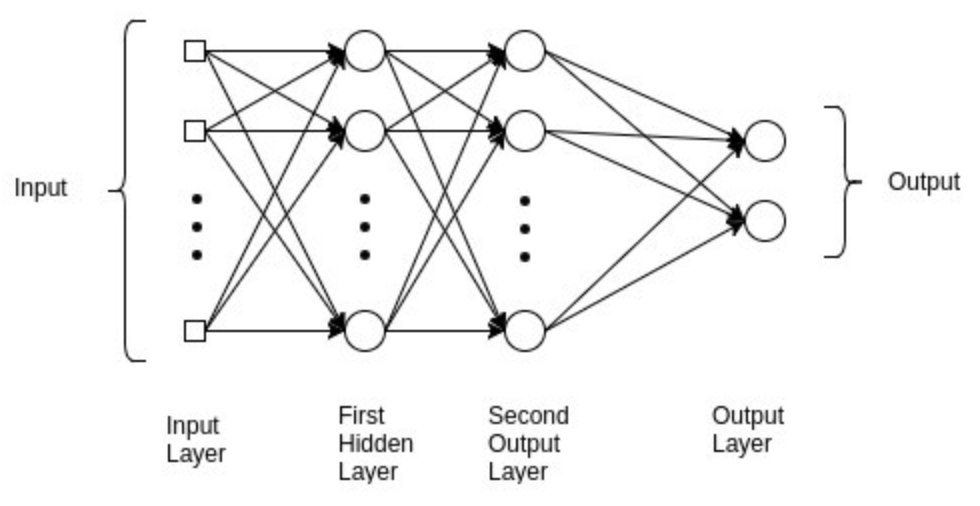
\includegraphics[width=.9\linewidth]{images/MLP_architecture.png}
\caption{Ejemplo de una red neuronal perceptron multicapa.}
\label{fig:MLP_architecture}
\end{center}
\end{figure}

Se decidió utilizar este modelo a modo de \textit{baseline}, y para determinar cuál estrategia de representación de palabras del trabajo de \cite{iacobacci-etal-2016-embeddings} funcionaba mejor. La capa de entrada del modelo toma una palabra representada a través de un vector, resultante de haber aplicado alguna de las estrategias citadas en la sección \ref{sec:palabraEtiqueta}. La capa de salida contiene cinco neuronas, ya que se cuenta con cinco clases: PER - LOC - ORG - MISC - O, posteriormente se aplica la función de activación softmax que asigna la salida no normalizada a una distribución de probabilidad sobre las clases de salida.

\subsection{Redes convolucionales en amplitud}\label{sec:cnn:wide}

\begin{figure}[ht!]
\begin{center}
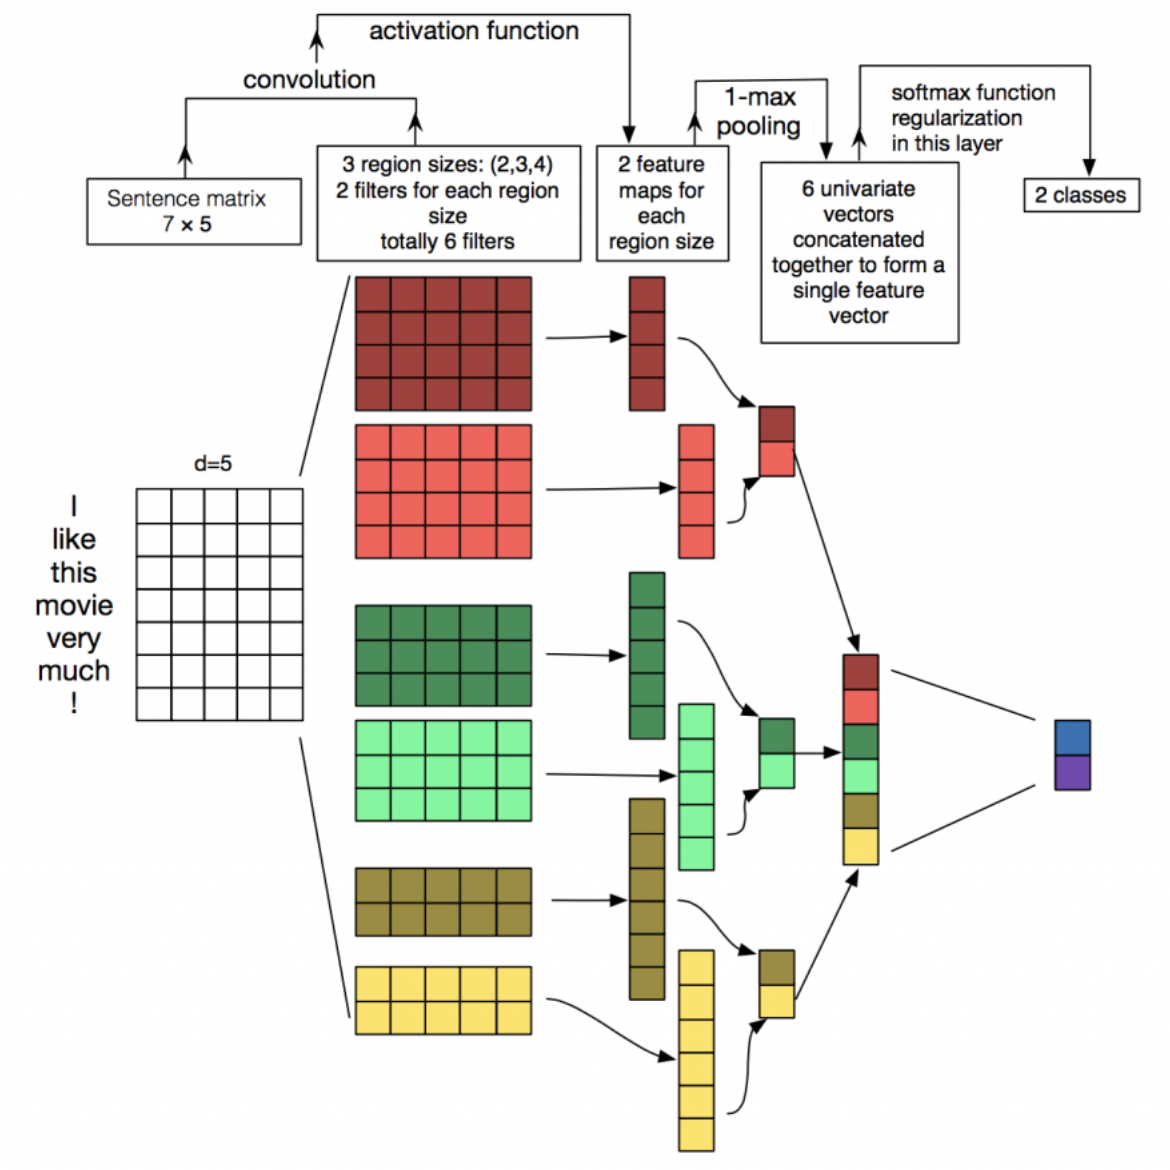
\includegraphics[width=.9\linewidth]{images/CNN_wide_NLP.png}
\caption{Ejemplo de una red convolucional en amplitud para análisis de sentimiento.}
\label{fig:CNN_wide_architecture}
\end{center}
\end{figure}

La entrada de la mayoría de los modelos que realizan tareas de procesamiento de lenguaje natural son oraciones o documentos representados en una matriz. Cada fila de la matriz corresponde a un \textit{token}, típicamente una palabra, pero también podría ser un carácter, representado a través de un vector.

Al aplicar los filtros de las convoluciones, usualmente los mismos se deslizan sobre las filas completas de la matriz (palabras). Por lo tanto, el ancho de nuestros filtros suele ser el mismo que el ancho de la matriz de entrada. La altura es lo que puede variar, tomando ventanas de \textit{n} palabras a la vez.

La Figura \ref{fig:CNN_wide_architecture} muestra un ejemplo de esta arquitectura\footnote{\url{http://www.wildml.com/2015/11/understanding-convolutional-neural-networks-for-nlp/}}. Se toman filtros de alturas 2, 3 y 4 y se supone un \textit{stride} (desplazamiento del filtro en cada paso) igual a 1. Luego de la convolución se aplica una función de activación y se obtienen distintos vectores que contienen información sobre la sentencia original. Posteriormente se aplica una capa de \textit{max pooling} cuyo objetivo es reducir la dimensionalidad pero con la promesa de mantener la información más relevante. Finalmente se construye un único vector al concatenar los vectores resultantes y se aplica una función de activación softmax a la capa densa de salida para realizar la clasificación correspondiente.

\subsection{Redes convolucionales en profundidad}\label{sec:cnn:deep}

Una alternativa al modelo de redes convolucionales en amplitud que también le permite a las representaciones intermedias obtener información sobre el contexto de la sentencia es el modelo de redes convolucionales en profundidad.

La idea es hacer crecer el campo receptivo a medida que se apilan más y más capas convolucionales. Esto significa que, de forma predeterminada, cada paso en la representación de la convolución ve toda la entrada en su campo receptivo.

En la Figura \ref{fig:CNN_depth_architecture} se puede ver como al agregar más capas se incrementa el campo receptivo\footnote{\url{https://medium.com/@TalPerry/convolutional-methods-for-text-d5260fd5675f}}. Esto significa que dada una profundidad suficiente, nuestra red podría mirar toda la capa de entrada, a través de unas pocas abstracciones.

\begin{figure}[hb]
\begin{center}
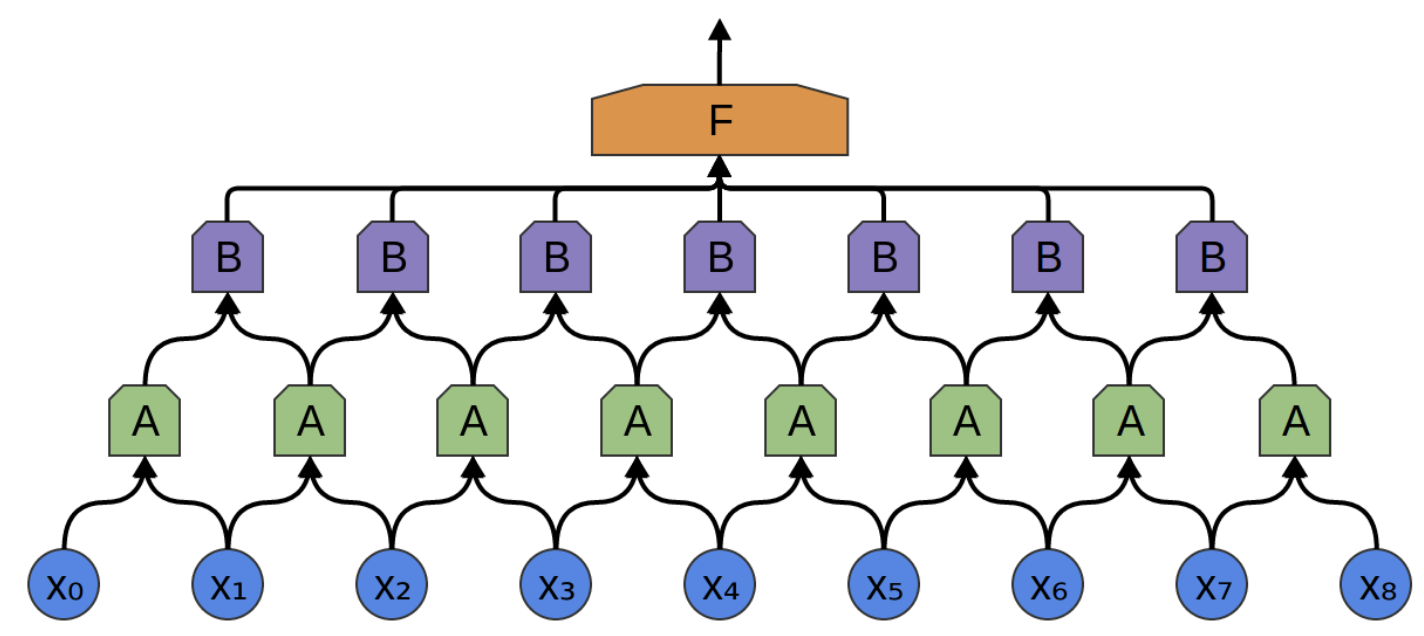
\includegraphics[width=.9\linewidth]{images/CNN_depth_NLP.png}
\caption{Ejemplo de una red convolucional en profundidad.}
\label{fig:CNN_depth_architecture}
\end{center}
\end{figure}

\subsection{Redes neuronales en escalera}\label{sec:ladder_net}

La idea detrás de las redes neuronales en escalera es entrenar simultáneamente una red neuronal del tipo 
\textit{feed-forward} (como lo son la red perceptrón multicapa y las redes convolucionales) junto con un 
autoencoder con pesos compartidos. La red se entrena aprendiendo dos objetivos diferentes: uno supervisado, 
dado por el error de predicción de los datos etiquetados; y otro no supervisado, dado por el error de 
reconstrucción de los datos sin etiquetar.

En el presente trabajo, se exploró el uso de un parámetro extra sobre la función de costo de la red en escalera original. Al factor no supervisado de la función de costo se lo multiplica por un parámetro $\mu$ que viene a representar la relevancia de la tarea no supervisada en el modelo. La función de costo final es:

\[
Cost = \text{supervised\_cost} + \mu ~ \text{unsupervised\_cost}
\]

La estructura del modelo es un autoencoder con \textit{skip connections} desde el codificador hacia 
el decodificador y la tarea de aprendizaje es similar a los autoencoders de eliminación de ruido popularmente 
conocidos como \texit{denoising autoencoders} pero en este caso dicha tarea se aplica a cada capa, no solo a 
las entradas. Las \textit{skip connections} liberan la presión de representar  los detalles en las capas más 
altas del modelo porque a través de estas conexiones el decodificador puede recuperar cualquier detalle 
descartado por el codificador. Una descripción más detallada de este modelo se encuentra en la sección 
\ref{sec:related_work_ladder} como así también remitimos al lector a \cite{DBLP:journals/corr/RasmusVHBR15}.